\documentclass[spanish,notitlepage,letterpaper, 12pt]{article}
\usepackage[spanish]{babel} 
\usepackage{amsmath}
\usepackage{amsfonts}
\usepackage{amssymb}
\usepackage{graphicx}
\usepackage{geometry}      
\geometry{letterpaper}                  
\usepackage{epstopdf}
\usepackage{fancyhdr} % Paquete para encabezados y pies de pag
\usepackage{color}
\usepackage{placeins}
\usepackage{csquotes}
\usepackage{textcomp}
\usepackage{gensymb}
\usepackage{lipsum}

\pagestyle{fancy}
\chead{\bfseries Informe 3 - Grupo C1B. Subgrupo 2} 
\rhead{5 de Mayo de 2023}
\cfoot{Universidad Industrial de Santander} 
\rfoot{\thepage} 

\voffset = -0.25in 
\textheight = 8.0in 
\textwidth = 6.5in
\oddsidemargin = 0.in
\headheight = 20pt 
\headwidth = 6.5in
\renewcommand{\headrulewidth}{0.5pt}
\renewcommand{\footrulewidth}{0,5pt}
\begin{document}
\begin{titlepage}
    \begin{center}
        
\includegraphics[width=0.4\textwidth]{../general-images/uis-logo.png}
        
        \vspace{0.5cm}
        \LARGE
        \textbf{Estudio del comportamiento del circuito RLC y el fenómeno de resonancia}
        
        \vspace{0.5cm}
        \large
        Informe 4
        
        \vfill
        
        \textbf{Daniel Esteban Vargas Reyes.} Estudiante - Geología\\
        \textbf{Nicolás Andrés Ramírez Calderón.} Estudiante - Ingeniería de Sistemas\\ 
        \textbf{Rodolfo Valentín Muñoz Vega.} Estudiante - Ingeniería Química\\

        \vspace{1.0cm}
        Presentado a la docente:
        
        \textbf{Zayda Paola Reyes Quijano}
        
        \vfill
        
        Escuela de Física - Física III\\
        Universidad Industrial de Santander\\
        Bucaramanga, Santander, Colombia\\
        20 de Mayo de 2023        
    \end{center}
\end{titlepage}

\tableofcontents

\newpage

\section{Resumen}
\lipsum[1]
\section{Introducción}
En la cotidianidad, los fenómenos físicos tienen mucho menos de ideales que de curiosos.
Si bien los sucesos cotidianos parecen responder a unas leyes que solemos describir con fórmulas matemáticas, rara vez se ajustan a la perfección a dichas fórmulas. En un movimiento oscilatorio sucede algo parecido.\par
\bigskip
Hasta el momento, nuestros esfuerzos se han centrado en entender un movimiento oscilatorio en ausencia de fricción o aquellas que describen un movimiento sub-amortiguado. Pero también es relevante entender y aplicar conceptos sobre las diferentes oscilaciones amortiguadas y las forzadas.\par
\bigskip
En este proyecto de investigación se estudió la variación de la amplitud del
movimiento amortiguado en función del tiempo para diferentes constantes de
amortiguamiento y la amplitud del movimiento forzado en función de la frecuencia de la
fuerza externa para diferentes constantes de amortiguamiento.
\subsection{Marco teórico} \label{I.MT}
\subsubsection{Péndulo de Pohl}
El péndulo de Pohl consiste en una rueda de metal con momento de inercia $I$ que
oscila (Fig. \ref{fig:1} y un resorte helicoidal que produce un momento de torsión restaurador cuando la cuerda gira. \eqref{eq:1}
\begin{align}\label{eq:1}
    M=-K\theta
\end{align}
La situación descrita produce un movimiento oscilatorio que tiende a llevar al péndulo a la posición de equilibrio.
\newpage
\begin{figure}[ht]
    \centering
    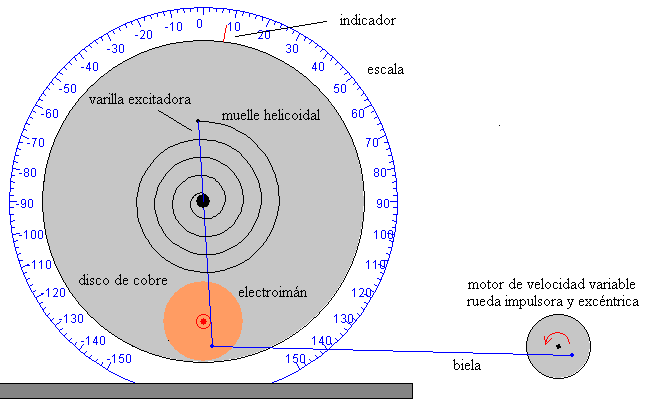
\includegraphics[width=10.0cm]{images/pendulo-pohl.png}
    \caption{\textit{Montaje del péndulo de Pohl}}
    \label{fig:1}
\end{figure}
Debido a la fricción, la amplitud disminuye con el tiempo generando un movimiento oscilatorio amortiguado. En el péndulo, el amortiguamiento se realiza pasando la rueda de metal a través del campo magnético de un electroimán y como resultado se genera en el disco una corriente ``parásita''. De modo
que el momento de las fuerzas que ejerce el campo magnético sobre las corrientes es proporcional a la velocidad angular de la rueda y va en sentido contrario.\par
\bigskip
El movimiento que realiza el péndulo de Pohl puede describirse mediante una ecuación diferencial lineal de segundo órden \eqref{eq:2}. \cite{serway_jewett_2017}
\begin{align}\label{eq:2}
    \ddot{\theta}+\beta\dot{\theta}+{\omega_0}^2\theta=0
\end{align}
De la ecuación \eqref{eq:2}, la constante de amortiguamiento $\gamma=\frac{\beta}{2I}$, la frecuencia natural del oscilador $\omega_0=\sqrt{\frac{k}{I}}$, mientras $I$ representa el momento de inercia del disco y $K$ la constante de restauración del resorte helicoidal.\par
\bigskip
Para este tipo de movimientos la frecuencia depende de la frecuencia natural del sistema así como de la constante de amortiguamiento $\gamma$. \eqref{eq:3}
\begin{align}\label{eq:3}
    \omega=\sqrt{{\omega_0}^2-\gamma^2}
\end{align}
Por otra parte, la solución de la ecuación diferencial \eqref{eq:2} tiene la forma de una multiplicación de fuciones; una exponencial y una sinusoidal. \eqref{eq:4}
\begin{align}\label{eq:4}
    \theta(t)=\theta_0e{-\gamma t}\cos{\omega t}
\end{align}
Para la ecuación \eqref{eq:4} $\theta_0$ es el ángulo inicial de rotación en el instante $t_0$.\par
\bigskip
Es importante notar que la relación entre las variables que afectan la frecuencia describen tres tipos de movimientos:
\begin{enumerate}
    \item Cuando ${\omega_0}^2>\gamma^2$, se tiene un \textbf{movimiento amortiguado}, o sea que el sistema oscila con amplitud decreciente.
    \item Cuando ${\omega_0}^2=\gamma^2$, se tiene un \textbf{amortiguamiento crítico}, o sea que el sistema vuelve a su posición de equilibrio sin oscilar cuando se le desplaza.
    \item Cuando ${\omega_0}^2<\gamma^2$, se tiene un \textbf{movimiento sobreamortiguado}, en este caso no hay oscilación, pero el sistema retorna a su punto de equilibrio más lento que cuando está críticamente amortiguado.
\end{enumerate}
\subsubsection{Oscilaciones forzadas}
La ecuación \eqref{eq:2} puede ser utilizada para las oscilaciones forzadas con la diferencia de que ahora se ejerce una fuerza externa periódica, luego la ecuación tomaría la forma de \eqref{eq:5}.
\begin{align}\label{eq:5}
    \ddot{\theta}+\beta\dot{\theta}+{\omega_0}^2\theta=F_0\cos{(\omega t)}
\end{align}
donde $F_0=\frac{M_0}{I}$ y cuya solución general es la misma que la del movimiento libre añadiendole una solución partícular de la forma \eqref{eq:6}.
\begin{align}\label{eq:6}
    \theta=A_F\cos{(\omega t - \delta)}
\end{align}
donde la amplitud del movimiento forzado $A_F$ depende de la magnitud del momento aplicado y de la frecuencia externa $\omega$ tal como se muestra en la ecuación \eqref{eq:7}.
\begin{align}\label{eq:7}
    A_F=\frac{F_0}{\sqrt{(\omega^2-{\omega_0}^2)^2}+\gamma^2\omega^2}
\end{align}
mientras que el desfase entre el momento externo y la oscilación se puede ver en la ecuación \eqref{eq:8}.
\begin{align}\label{eq:8}
    \delta=\arctan{\left(\frac{2\gamma\omega}{{\omega_0}^2-\omega^2}\right)}
\end{align}
En este caso, existe una frecuencia para la cual la amplitud es máxima, esta es llamada \textbf{frecuencia de resonancia} y se expresa de la forma \eqref{eq:9}.
\begin{align}\label{eq:9}
    \omega_R=\sqrt{{\omega_0}^2-2\gamma^2}
\end{align}
Según la ecuación \eqref{eq:9} se hace visible que en el caso de que no exista amortiguamiento, la frecuencia de resonancia corresponde a
la frecuencia natural y la amplitud tenderá al infinito; para frecuencias altas la amplitud
tenderá a cero y para muy bajas frecuencias la amplitud tenderá a $F_0$.
\section{Metodología}
El desarrollo del proyecto se realizó en tres etapas o fases metodológicas, en las
cuales se procedió a la recolección de los datos y posteriormente su respectivo procesamiento.
En la primera fase se obtuvieron los datos de las amplitudes y el tiempo de $3$ oscilaciones
del movimiento débilmente amortiguado con el fin de demostrar que ésta decae
exponencialmente con el tiempo. Por otra parte, también se observaron los movimientos
críticamente amortiguados y sobre amortiguados. En la segunda fase se registrarón los
valores de la amplitud en función de la frecuencia del movimiento forzado para diferentes
constantes de amortiguamiento y se obtuvo la frecuencia natural del oscilador.
\subsection{Materiales}
\begin{enumerate}
    \item Péndulo de Pohl.
    \item Fuente de alimentación.
    \item Fuente plug-in para el péndulo de torsión.
    \item Amperímetro.
    \item Voltímetro.
    \item Cables de conexión.
    \item Cronómetro.
\end{enumerate}
\subsection{Fase 1} \label{M.F1}
En esta primera fase se determinó la amplitud del movimiento amortiguado
en función del tiempo. Para esto, se aplicó una corriente continua a las bobinas para
generar la fuerza que amortigua las oscilaciones en el péndulo de Pohl (a mayor corriente
mayor amortiguamiento). Luego, se desplazó el indicador del péndulo hasta una posición límite y se registraron las
amplitudes sucesivas del péndulo (positivas y negativas) correspondientes a
la corriente utilizada. Finalmente, se repitió el procedimiento anterior para otra corriente
y se registraron los datos.
\subsection{Fase 2} \label{M.F2}
En ésta fase se determinó el período del movimiento amortiguado. Para esto,
se ajustó en las bobinas la primera corriente utilizada en la fase anterior \ref{M.F1}. Luego, se
separó el péndulo hasta una amplitud inicial límite y se midió el tiempo de 3
oscilaciones tres veces. Posteriormente, se obtuvo el tiempo promedio y el período promedio
del movimiento. Por último, se repitió el procedimiento anterior con la segunda
corriente y se registraron los datos.
\subsection{Fase 3} \label{M.F3}
En esta fase se observó el comportamiento de la amplitud en los
movimientos críticamente amortiguado y sobreamortiguado. Aquí fue necesario ajustar el
valor de la corriente aumentándola hasta obtener un movimiento críticamente amortiguado. Luego, se determinó el tiempo que tarda el péndulo desde que se libera hasta que alcanza la posición de
equilibrio. Después, se siguieron aumentando los valores
de la corriente hasta alcanzar un amortiguamiento que generó un movimiento sobre
amortiguado. Posteriormente, se midió el tiempo que tarda el péndulo en realizar el movimiento
hasta alcanzar la posición de equilibrio. Por último, se registrarán los valores de corriente
y tiempo para cada movimiento.
\subsection{Fase 4}
En esta fase se estudió la respuesta forzada del péndulo de Pohl. El procedimiento realizado fue:
\begin{enumerate}
    \item Se determinó el valor de la amplitud del
péndulo para una corriente de $0A$ a una frecuencia $f$ 
    \item Se realizó el mismo procedimiento anterior variando las frecuencias aumentando de cinco en cinco los valores de la perilla tal como lo indicó la docente, fue importante tener en cuenta que para determinar el valor de la frecuencia fue necesario tomar el tiempo de 5 revoluciones del motor. 
    \item Se repitieron los pasos anteriores ajustando las dos corrientes utilizadas en la fase \ref{M.F1} para generar el movimiento forzado-amortiguado,
registrando nuevamente los datos de las amplitudes.
\end{enumerate}
Por último, se determinó cualitativamente la relación de fase entre el excitador y el
oscilador para cada frecuencia ajustada. Finalmente, se encontró la frecuencia natural
de oscilación del péndulo de Pohl, registrando el tiempo de las oscilaciones sin corriente y
sin fuerza externa.
\newpage
\section{Fase 5}
\begin{figure}[ht]
    \centering
    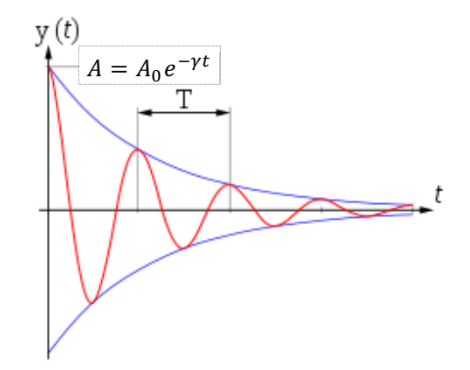
\includegraphics[width=10.0cm]{images/amplitud-vs-tiempo.png}
    \caption{\textit{Amplitud en función del tiempo para un movimiento sub-amortiguado.}}
    \label{fig:2}
\end{figure}

Se establecieron las funciones de la amplitud para el movimiento
débilmente amortiguado y para el movimiento forzado. Para esto, se realizó un análisis
de la gráfica de amplitud, $A(t)$ contra tiempo $t$ para las dos
corrientes utilizadas en el movimiento amortiguado. Posteriormente, sobre los puntos
experimentales se realizó un ajuste exponencial de la forma: $A_0e^{-\gamma t}$. (Fig. \ref{fig:2})
\section{Tratamiento de datos} \label{TD}
\section{Análisis de resultados}
La toma de datos fue parte fundamental del proceso de investigación y para la comparación con los resultados esperados con los obtenidos. Inicialmente se tomaron unas amplitudes positivas y negativas con diferentes coeficientes de amortiguamiento, las cuales dieron cifras aproximadas a lo que se
esperaba como equipo de trabajo, posteriormente se midió la frecuencia del motor, siendo que los resultados de las amplitudes con diferentes corrientes de frenados, no fuesen muy diferentes entre sí.
\section{Conclusiones}
Cerrando el proceso de experimentación e investigación se puede decir que se cumplieron con los objetivos propuestos, principalmente con el entender como funciona un movimiento armónico amortiguado forzado y como varía en función del coeficiente de amortiguamiento o la corriente de frenado en este caso. Tambien se concluyó que la frecuencia del motor es mayor en cuanto se aumenta la posición del dial, y teniendo un dato extra de que cuando se encuentra aproximadamente en 25 la posición del dial, el movimiento se encuentra en resonancia.
\section{Referencias} 
\bibliographystyle{unsrt}
\bibliography{../general-references/references}
\end{document}
